\documentclass[12pt, oneside]{article}
\usepackage[letterpaper, margin=1in]{geometry}
\usepackage[english]{babel}
\usepackage[utf8]{inputenc}
\usepackage{amsmath}
\usepackage{amsfonts}
\usepackage{amssymb}
\usepackage{tikz}

\usepackage{fancyhdr}
\pagestyle{fancy}
\fancyhf{}
\rhead{Name: \hspace{1.5in} }
\lhead{BECA / Dr. Huson / 11.1  Math SL  \\* 26 March 2018 \\* Do Now Quiz}

\vspace{1cm}

\renewcommand{\headrulewidth}{0pt}

\title{Worksheet and test template}
\author{Chris Huson}
\date{March 2018}

\begin{document}

\subsubsection*{%\\* Open book, open note. Use the formula sheet. \\* 
Answer in space provided. Show work.}

\begin{enumerate}

\vspace{0.5 cm}

\subsubsection*{Graphing exponential functions}
\item Graph $g(x)=15(1.15)^{2x}+25$ on the set of axes below.
\begin{center}
    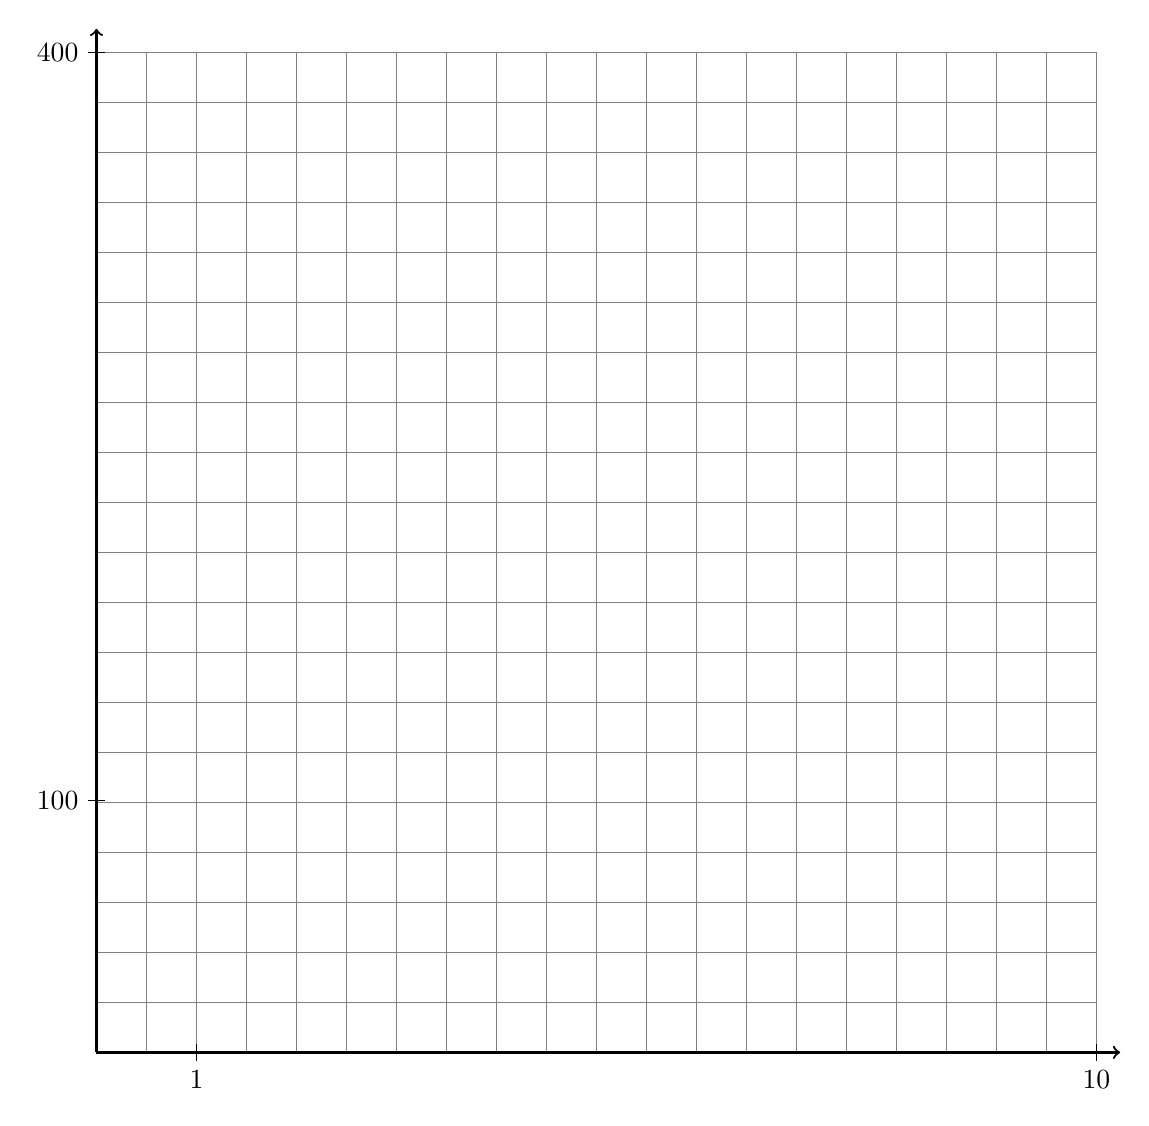
\begin{tikzpicture}
    \draw[step=0.25in,gray,very thin] (0,0) grid (12.7,12.7);
    \draw[thick,->] (0,0) -- (13,0); node[anchor=north west] {x};
    \draw[thick,->] (0,0) -- (0,13); node[anchor=south east] {y};
    \foreach \x in {1.27} \draw (\x cm,3pt) -- (\x cm,-3pt) node[anchor=north] {$1$};
    \foreach \x in {12.7} \draw (\x cm,3pt) -- (\x cm,-3pt) node[anchor=north] {10};
    \foreach \y in {3.2} \draw (3pt,\y cm) -- (-3pt,\y cm) node[anchor=east] {100};
    \foreach \y in {12.7} \draw (3pt,\y cm) -- (-3pt,\y cm) node[anchor=east] {400};
    \end{tikzpicture}
\end{center} %Alg2 Regents Jun2017

\item Is the function an example of exponential growth or exponential decay?
\begin{enumerate}
    \item Support your answer with evidence from the graph.\\*[25pt]
    \item Give an algebraic argument to explain your answer. 
\end{enumerate}

\end{enumerate}
\end{document}